\section{\K 电路中的暂态分析}
\begin{definition}[暂态过程]
    \Par 若电路中含有电感元件或电容元件,当电路接通、断开或电路参数改变,这种电路一般需要经过一定短暂时间才能重新到达稳态,期间的过渡状态被称作\textbf{暂态过程}.
\end{definition}
\hl{换路}:电路接通、断开、改接以及参数和电源发生突变等情况.

出现暂态过程的\hl{原因}:
\begin{enumerate}
    \item 外因:换路
    \item 内因:电路中有储能元件:电容C或电感L
\end{enumerate}
\Par 暂态过程伴随着储能元件的储能或放能,电容将电路的能量转换为静电能,电感将电路的能量转换为磁场能.由于储能或放能需要时间(不然功率会趋于无穷大),因此暂态过程会经过一段时间.由实验可以知道,在暂态过程中,电容电压随时间的变化和电容电流随时间的变化如图所示
\begin{figure}[htbp]
    \centering
    \begin{minipage}{0.48\textwidth}
        \centering
        \includegraphics[width=0.6\textwidth]{uc.png}
        \caption{$u_C-t$图}
    \end{minipage}
    \begin{minipage}{0.48\textwidth}
        \centering
        \includegraphics[width=0.6\textwidth]{il.png}
        \caption{$i_L-t$图}
    \end{minipage}
\end{figure}

可见,$u_C$与$i_L$随时间的变化符合指数模型.
\begin{definition}[一阶线性电路]
    \Par 仅含一个储能元件或可等效为一个储能元件,且可以用一阶微分方程描述的线性电路,称作\textbf{一阶线性电路}.
\end{definition}
根据电路响应的变化情况,我们将暂态过程分类:
\begin{enumerate}
    \item \textbf{零输入响应}:初状态$f\left( 0^+ \right) \ne 0$且末状态$f\left( \infty \right) =0$的情况称作\textbf{零输入响应};
    \item \textbf{零状态响应}:初状态$f\left( 0^+ \right) =0$且末状态$f\left( \infty \right) \ne 0$的情况称作\textbf{零状态响应};
    \item \textbf{全响应}:初状态$f\left( 0^+ \right) \ne 0$且末状态$f\left( \infty \right) \ne 0$的情况被称作\textbf{全响应}.
\end{enumerate}

\begin{figure}[htbp]
    \centering
    \begin{minipage}{0.48\textwidth}
        \centering
        \includegraphics[height=0.18\textheight,width=0.65\textwidth]{零输入响应.pdf}
        \caption{零输入响应}
        \vspace{0.8cm}
    \end{minipage}
    \begin{minipage}{0.48\textwidth}
        \centering
        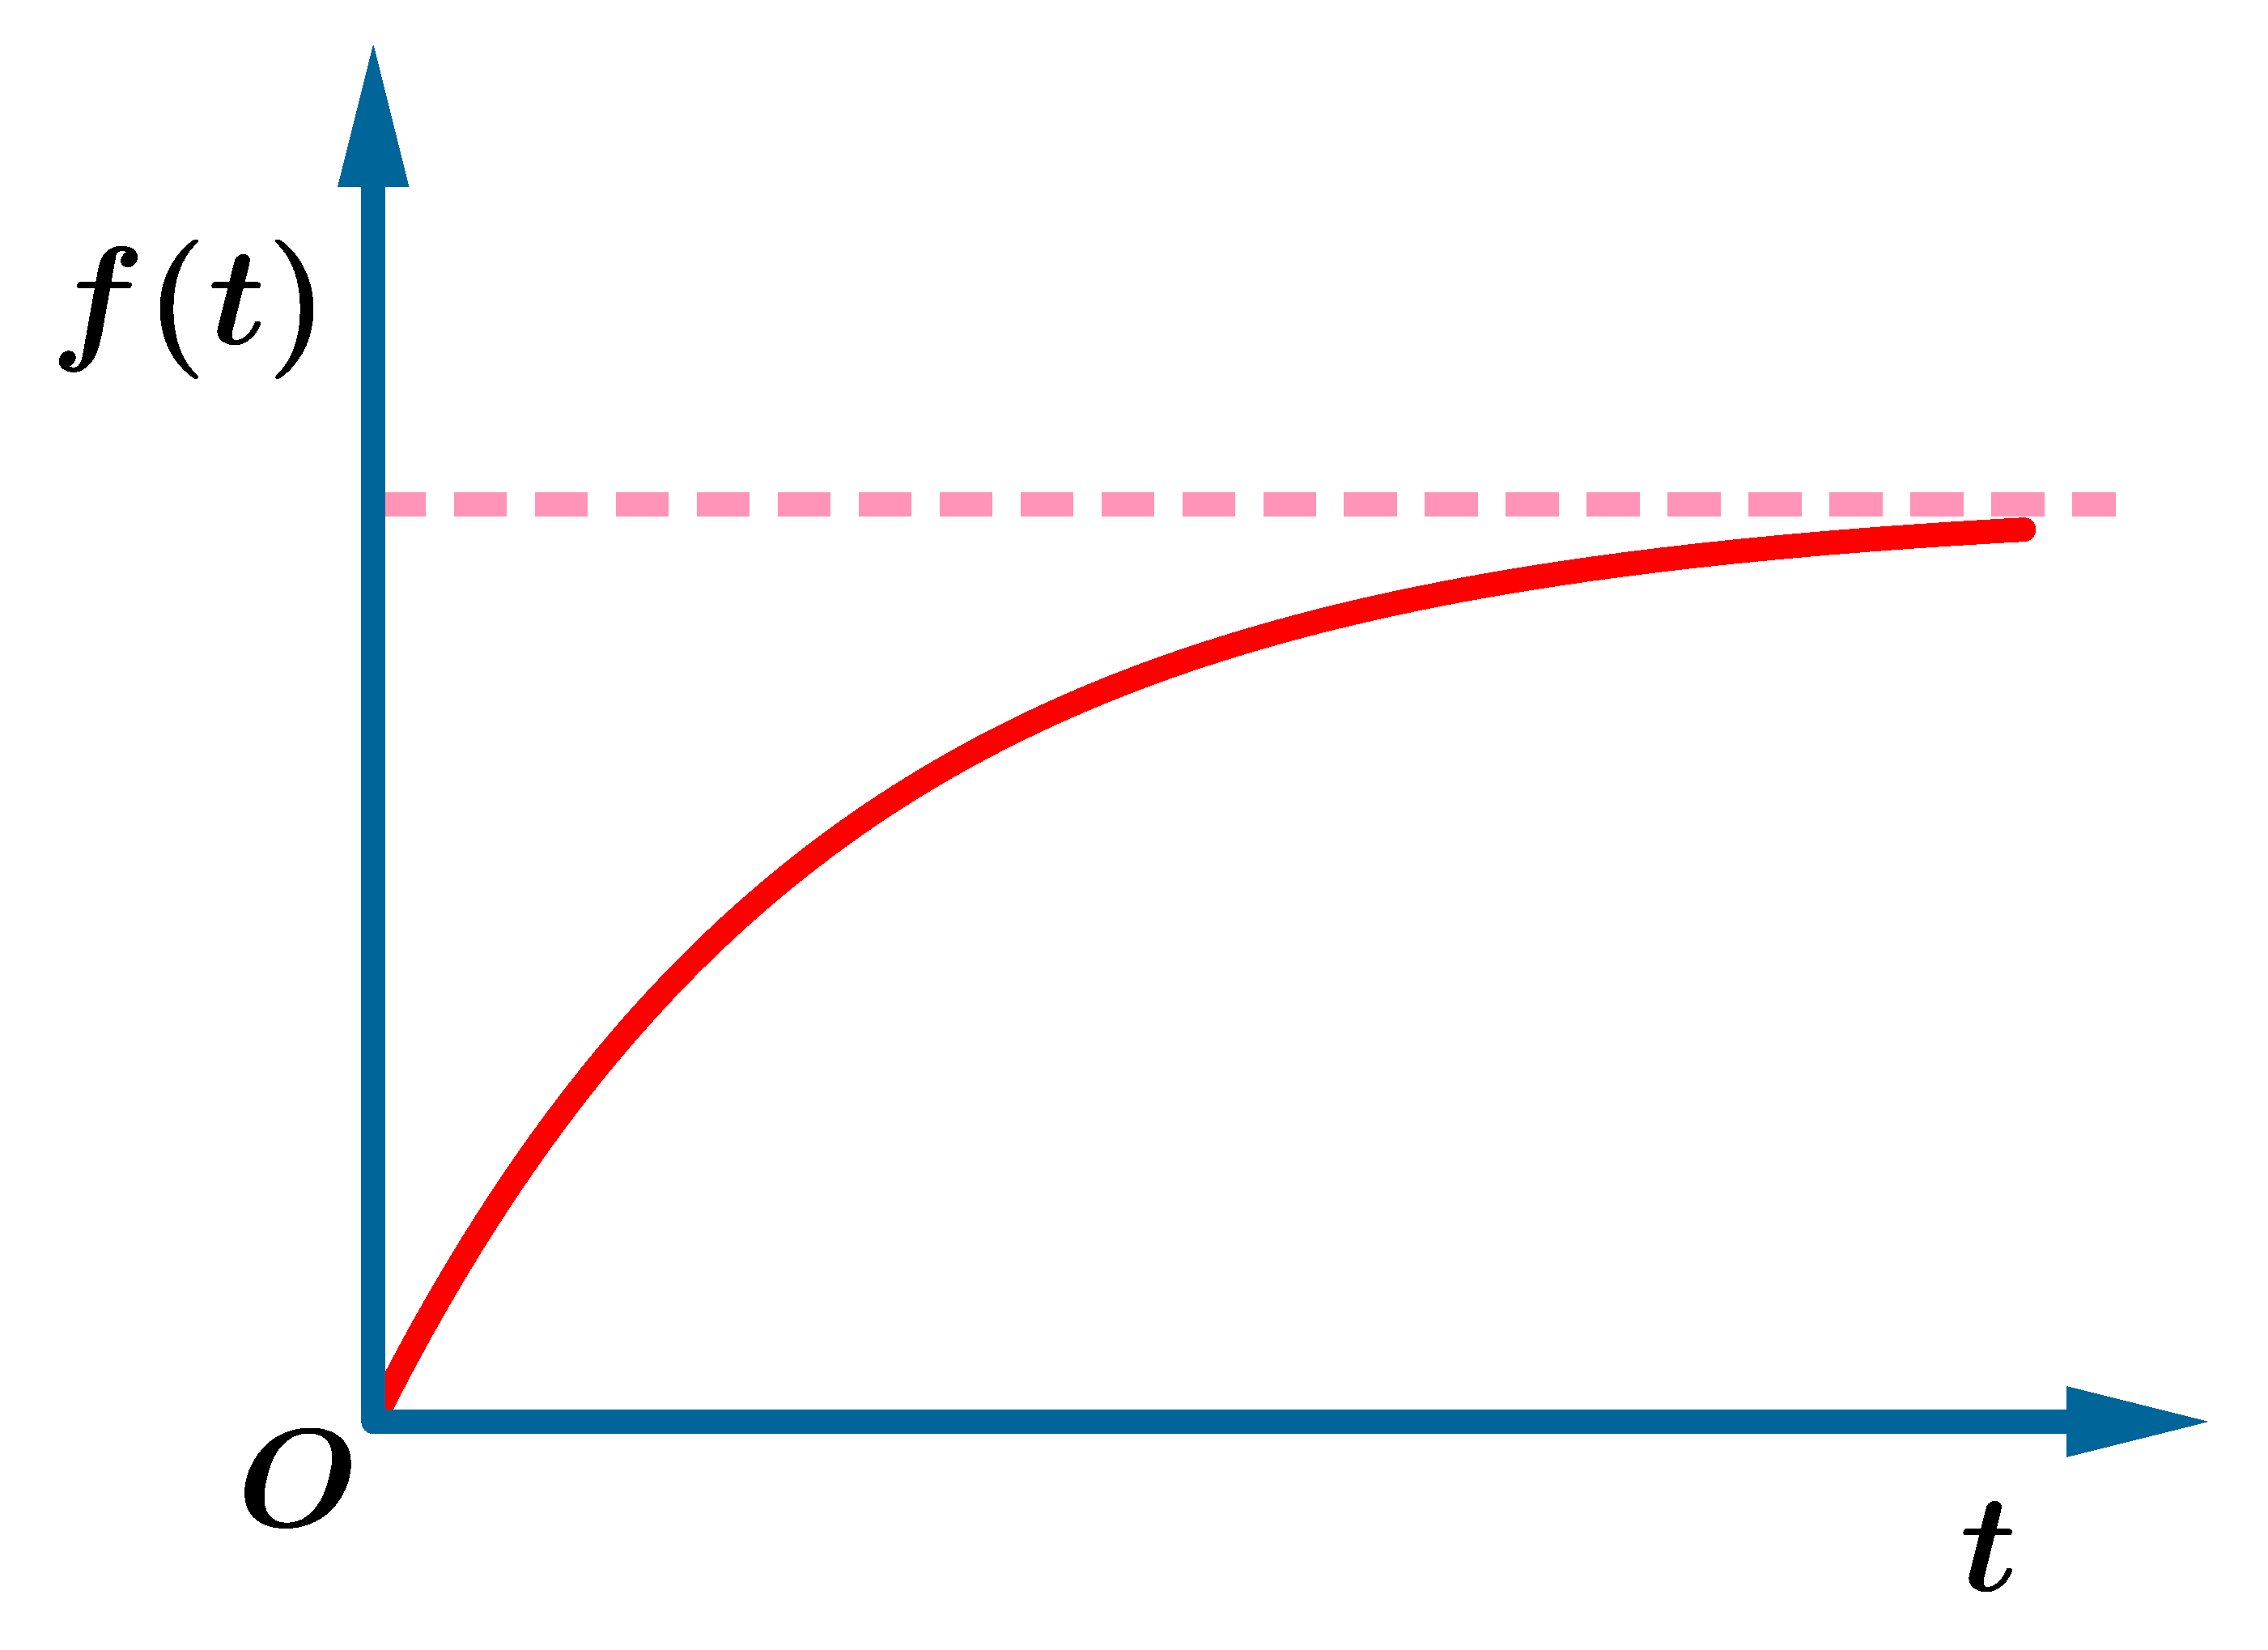
\includegraphics[height=0.18\textheight,width=0.65\textwidth]{零状态响应.pdf}
        \caption{零状态响应}
        \vspace{0.8cm}
    \end{minipage}
    \begin{minipage}{0.48\textwidth}
        \centering
        \includegraphics[height=0.18\textheight,width=0.65\textwidth]{全响应1.pdf}
    \end{minipage}
    \begin{minipage}{0.48\textwidth}
        \centering
        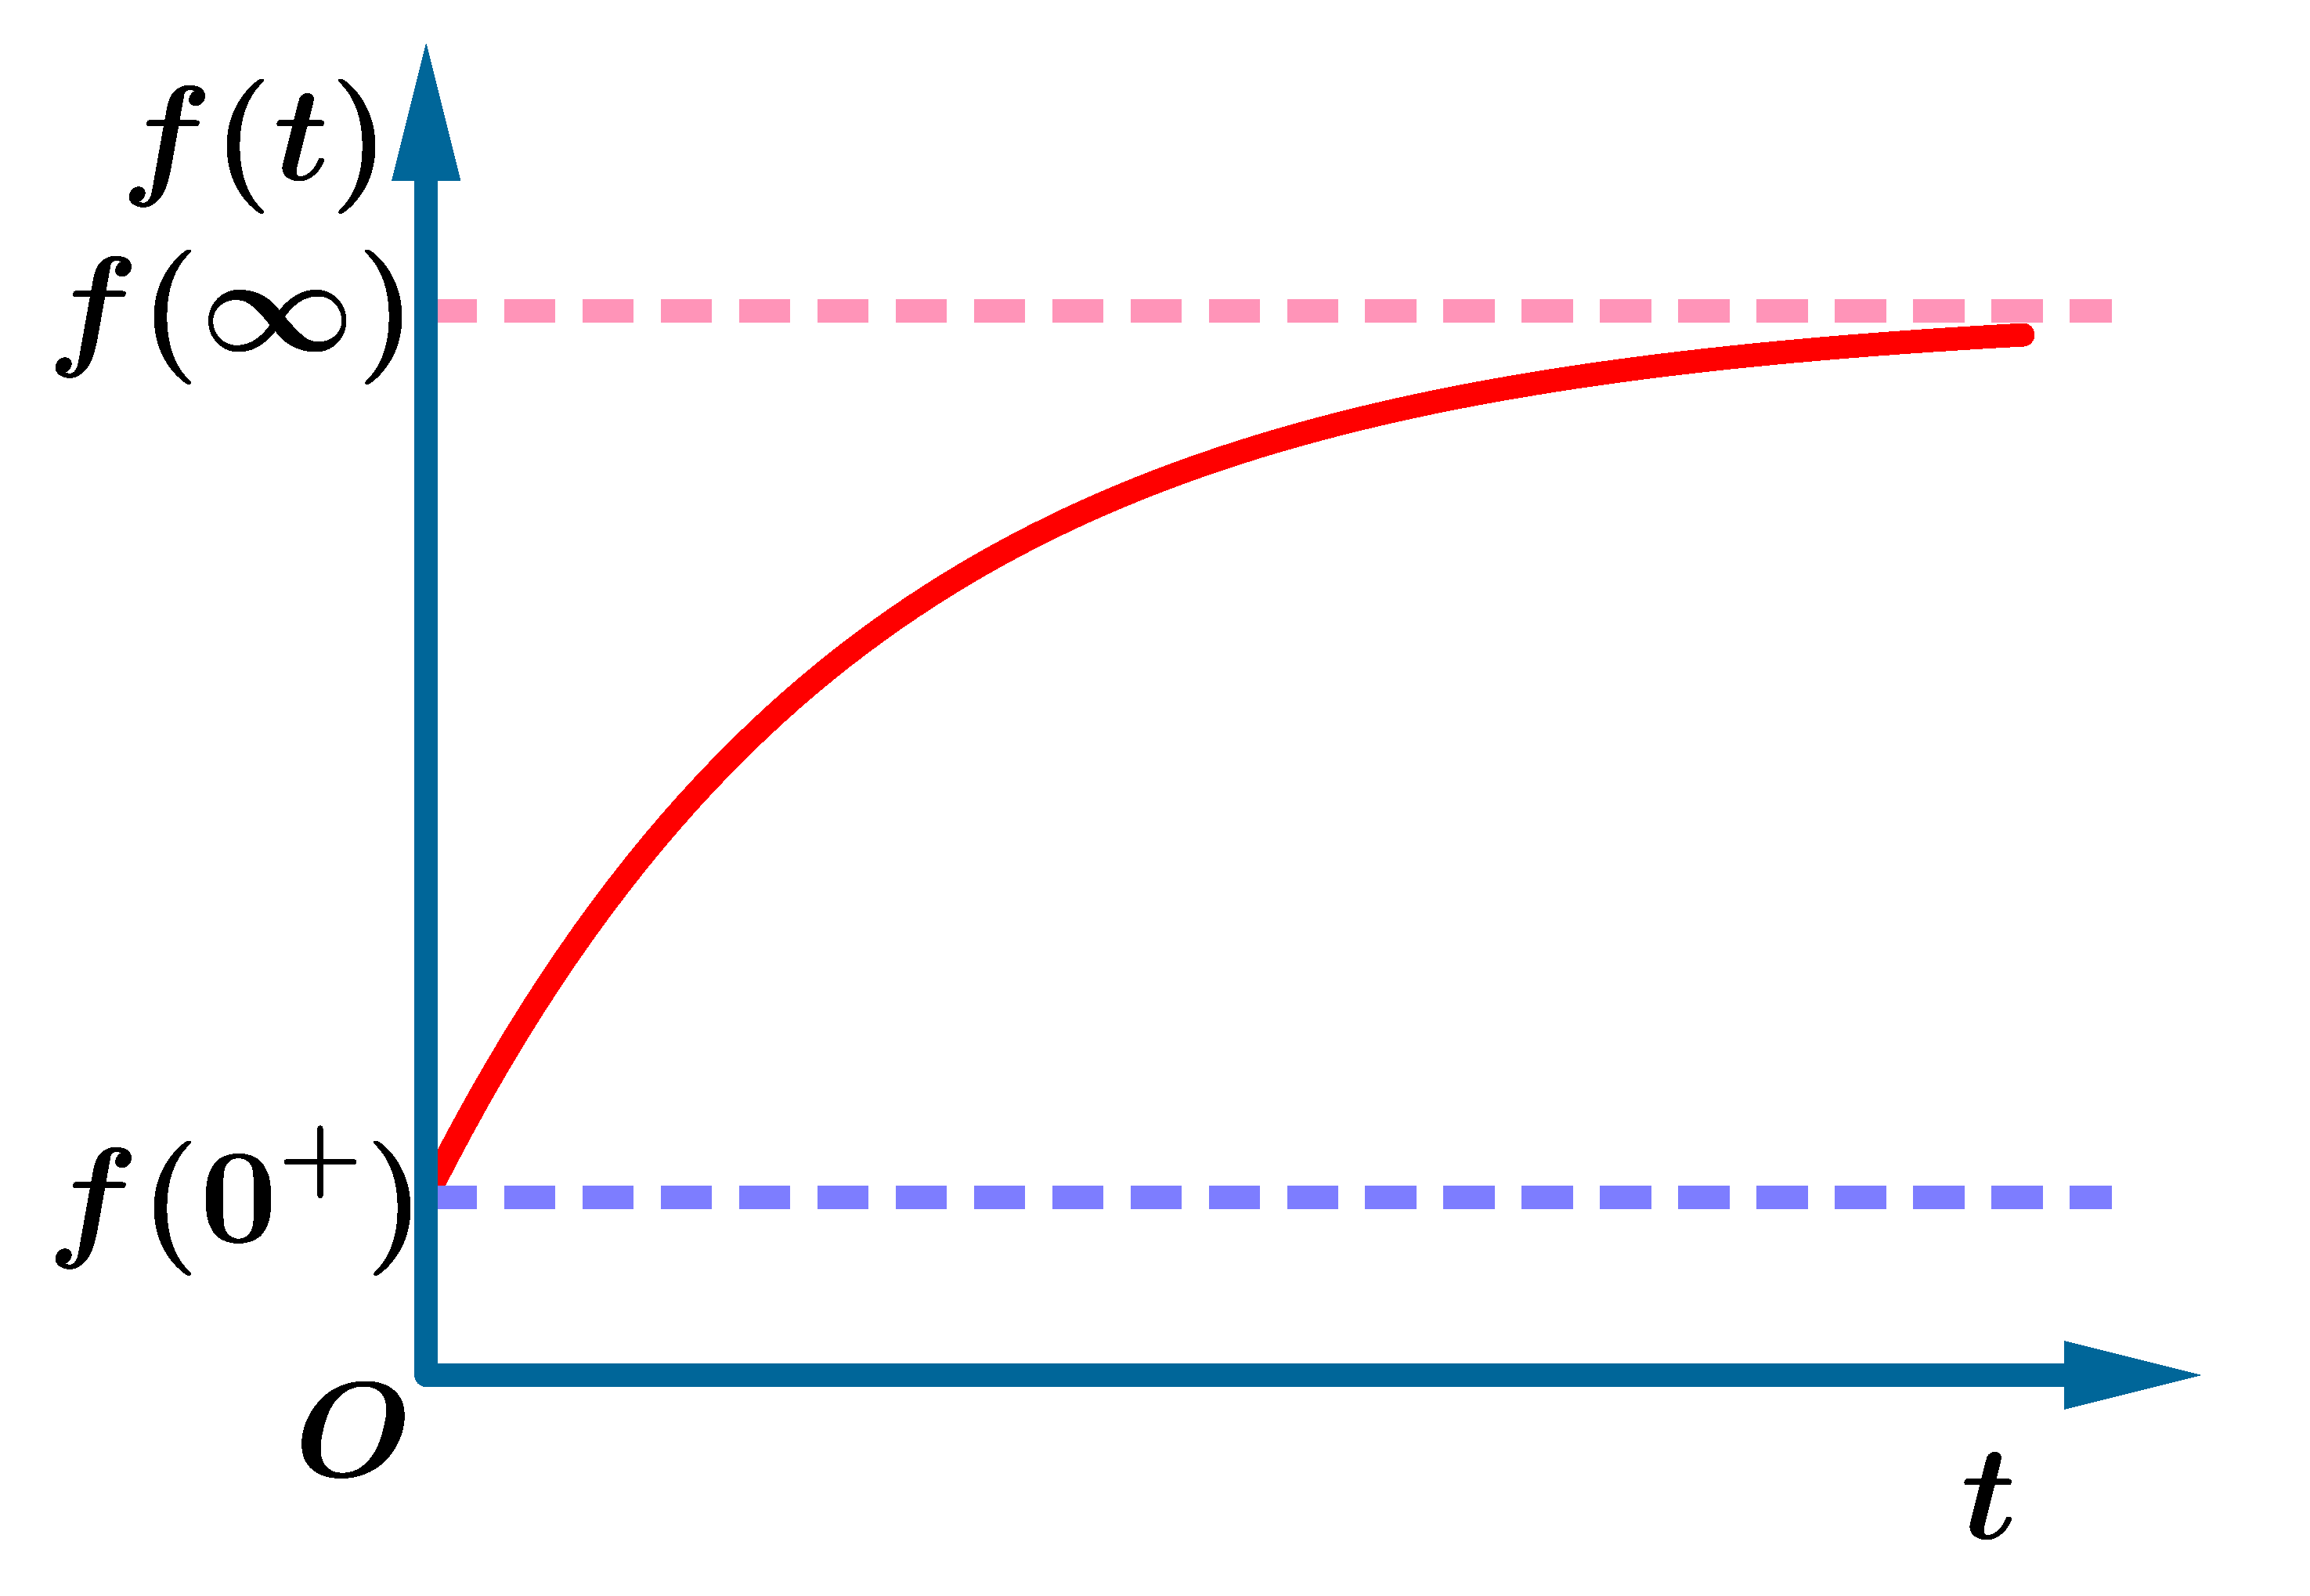
\includegraphics[height=0.18\textheight,width=0.65\textwidth]{全响应2.pdf}
    \end{minipage}
    \caption{全响应}
\end{figure}
根据分析,三种暂态过程的响应随时间的变化都可以用一个函数来表示
\begin{equation}\label{equ:暂态过程}
    f\left( t \right) =f\left( \infty \right) +\left[ f\left( 0^+ \right) -f\left( \infty \right) \right] e^{-\frac{t}{\tau}}
\end{equation}
其中$\tau $被称作时间常数.

由式\ref{equ:暂态过程}可知,如果我们也要确定一个暂态过程中响应随时间在每一刻的状况,那么必然要知道三个参量:
\begin{enumerate}
    \item[\circledtext{1}]  时间参量$\tau $;
    \item[\circledtext{2}]  初始值$f\left( 0^+ \right) $;
    \item[\circledtext{3}]  稳态值$f\left( \infty \right) $.
\end{enumerate}
\hl{时间参量$\boldsymbol{\tau } $}的值被定义为
\begin{equation*}
    \tau =\left\{ \begin{aligned}
        R_0C\,\, &,\text{电容电路}\\
        \frac{L}{R_0}\,\, &,\text{电感电路}\\
    \end{aligned} \right. 
\end{equation*}
其中$R_0$是将储能元件断开后形成的二端网络的等效内阻,但在实际的计算中,我们一般选用$\tau $的另一个定义:
\begin{definition}[时间参量$\tau $]
    \Par 时间参量$\tau $等于零输入响应中,响应衰减到初始值$f\left( 0^+ \right) \ne 0$的36.8\%或是零状态响应中,响应增长到到稳定值$f\left( \infty \right) $的63.2\%所需的时间.
\end{definition}
\Par 时间参量$\tau $是用来衡量\hl{暂态过程变化快慢}的参量,$\tau $越大,曲线变化越慢,响应达到稳态所需要的时间就越长.利用量纲分析,我们不难知道$\tau $的量纲为$\left[ \mathrm{T}^1 \right] $,单位为秒$\left( \cdot \mathrm{s} \right) $.

\Par 时间参量$\tau $的定义使得我们能够衡量暂态过程正在进行的阶段,因为不同的暂态过程达到稳态所需的时间不同,有的可能只需要几微秒,有的甚至要几百秒,但是如果我们用$\tau $来描述,我们就可以说“某暂态过程进行到了$3\tau $阶段”.

\Par 理论上,当$t\to \infty$时,我们称暂态过程\hl{结束};但在工程中,我们通常认为暂态过程进行到$3\tau \sim 5\tau $阶段时,暂态过程就基本结束了.

\Par 暂态过程的稳定值$f\left( \infty \right) $好求,重点在于暂态过程的初始值$f\left( 0^+ \right) $怎么求,这里我们有换路定理:
\begin{theorem}[换路定理]
    \Par 我们称$t=0$的时刻为\textbf{换路瞬间},$t=0^-$的时刻为\textbf{换路前瞬间},$t=0^+$的时刻为\textbf{换路后瞬间}.从$t=0^-$瞬间到$t=0^+$瞬间电感元件中的电流和电容元件上的电压不能跃变,即
    \begin{equation}
        \begin{aligned}
            u_C\left( 0^- \right) &=u_C\left( 0^+ \right)\\
            i_L\left( 0^- \right) &=i_L\left( 0^+ \right)
        \end{aligned}
    \end{equation}
    它被称作\textbf{换路定理}.
\end{theorem}
换路定理的提出也暗示我们有些参量是可以跃变的,例如电感元件中的电压和电容元件上的电流.

\begin{wrapfigure}[3]{r}{0.3\textwidth}
    \centering
    \includegraphics[width=0.3\textwidth]{暂态分析例题.pdf}
    \caption{例\ref{exm:暂态分析}用图}
    \label{fig:暂态分析例题}
\end{wrapfigure}
\begin{example}\label{exm:暂态分析}
    如图\ref{fig:暂态分析例题}所示,已知$U=6\mathrm{V}$,$R_1=1\mathrm{k}\Omega $,$R_2=2\mathrm{k}\Omega $,$C=3\mathrm{\mu F}$,在$t<0$时,开关$S$断开,$t=0$时刻开关闭合,试求:$u_C\left( t \right) $和$i_C\left( t \right) $.
\end{example}

\begin{solution}
    根据三要素法,我们要分别求出$\tau $、$f\left( 0^+ \right) $和$f\left( \infty \right) $.

    \begin{enumerate}
        \item[\circledtext{1}]  时间参量$\tau $
        
        \Par 我们断开电容$C$,将电路左边视为有源二端网络来

        %为了配合wrapfigure的奇怪判定而做出的无奈之举
        求它的等效电阻.
        \begin{equation*}
            R_0=\frac{1}{\frac{1}{R_1}+\frac{1}{R_2}}=\frac{1}{\frac{1}{1}+\frac{1}{2}}=\frac{2}{3}\mathrm{k}\Omega 
        \end{equation*}
        根据定义,我们可以求出
        \begin{equation}
            \tau =R_0C=\frac{2}{3}\cdot 10^3\times 3\cdot 10^{-6}=2\cdot 10^{-3}\mathrm{s}
        \end{equation}

        \item[\circledtext{2}]  初始值$f\left( 0^+ \right) $
        
        根据换路定理,我们不难知道
        \begin{equation}
            u_C\left( 0^+ \right) =u_C\left( 0^- \right) =6\mathrm{V}
        \end{equation}
        为了求换路后电流$i_C\left( 0^+ \right) $,由于换路后电容的电压保持稳定,因此我们可以将电容$C$视为电压源$u_C$,它的电压大小为$6\mathrm{V}$,方向上正下负.
        
        \Par 由此,不难分析得到,由于电压源$U$和电容$u_C$的负极用导线连接,因此它们等势,而电阻$R_1$两端分别用导线连接着$U$和$u_C$的正极,因此电阻$R_1$左端与$U$的正极等势,$R_1$右端与$u_C$的正极等势,由于
        \begin{equation*}
            U=u_C=6\mathrm{V}
        \end{equation*}
        因此电阻两端等势,没有电流流经它.因此$i_C$可仅由右边的孔分析得到,同时需要注意,我们规定的$i_C$的参考方向是顺时针的,而实际的$i_C$方向是逆时针的,因此我们需要加上负号以示方向的相反
        \begin{equation}
            i_C\left( 0^+ \right) =-\frac{u_C}{R_2}=-\frac{6}{2000}=-3\cdot 10^{-3}\mathrm{A}
        \end{equation}

        \item[\circledtext{3}]  稳态值$f\left( \infty \right) $
    
        稳态值易求,这里我们直接给出结果
        \begin{equation}
            \begin{aligned}
                u_C\left( \infty \right) &=4\mathrm{V}\\
                i_C\left( \infty \right) &=0\mathrm{A}
            \end{aligned}
        \end{equation}
    \end{enumerate}
    综上所述,我们根据通解公式给出最终答案
    \begin{equation*}
        \left\{ \begin{aligned}
            u_C\left( t \right) &=4+2e^{-500t}&&\mathrm{V}\\
            i_C\left( t \right) &=-3e^{-500t}&&\mathrm{mA}\\
        \end{aligned} \right.
    \end{equation*}
\end{solution}
\begin{remark}
    为了求出储能元件上可以跃变的响应参量,我们可以将换路后瞬间的电容视为电压源,其等效电压等于换路后瞬间电压$u_C\left( 0^+ \right) $;将换路后瞬间的电感视为电流源,其等效电流等于换路后瞬间电流$i_C\left( 0^+ \right) $.

    \Par 同时需要注意,三要素法的基础是通解公式
    \begin{equation*}
        f\left( t \right) =f\left( \infty \right) +\left[ f\left( 0^+ \right) -f\left( \infty \right) \right] e^{-\frac{t}{\tau}}
    \end{equation*}
    而通解公式来自于解微分方程得到的通解,所有一阶线性电路都可以用三要素法解决,但不要忘记它的本质是什么,在拓展到二阶(非)线性电路等更难的问题时,我们就需要用本质的原理来解决问题,换言之,一定要注意三要素法的\textbf{适用范围}!
\end{remark}
